\documentclass[../PhysicsFormulae.tex]{subfiles}
\begin{document}

\subsection{Equations of Continuity}
Within a tube of flow (lots of streamlines), conservation of mass dictates
\[ \rho_1 A_1 v_1 = \rho_2 A_2 v_2 \]
which equates the mass flux, reducing into
\[ A_1 v_1 = A_2 v_2 \]
for incompressible fluids, which is volume flux. \\
Generally these apply if there are no sources or sinks between the inlet and outlet. 

\subsection{Bernoulli's Equation}
Bernoulli's equation relates flow along a streamline, assuming no losses of mechanical energy.
\[ P + \frac{1}{2}\rho v^2 + \rho g h = \textrm{constant} \]
in which $P$ is the static pressure and $\frac{1}{2}\rho v^2$ is the dynamic pressure. 

\subsubsection{Venturi Meter}
The venturi meter measures flow speed through a pipe. Suppose said pipe decreases its diameter, before which fluid of density $\rho$ has speed $v_1$. Let us attach a barometer with one end at the original diameter and another at the new one, containing fluid of density $\rho'$. Bernoulli's equation tells us
\[ v_1 = A_2 \sqrt{\frac{2(\rho ' - \rho)gh}{\rho (A_1^2 - A_2^2)}} \]
where $h$ is the height differential in the barometer.

\subsubsection{Pitot Tube}
The pitot tube is used to measure flow speed of gas around it, and it works by attaching a manometer to a tube. One side of the manometer will have less static pressure because there is airflow, while the other does not, and thus the speed of the flow can be determined from the height differential:
\[ v = \sqrt{\frac{2\rho'gh}{\rho}} \]

\begin{figure}
\centering
\begin{minipage}{.5\textwidth}
  \centering
  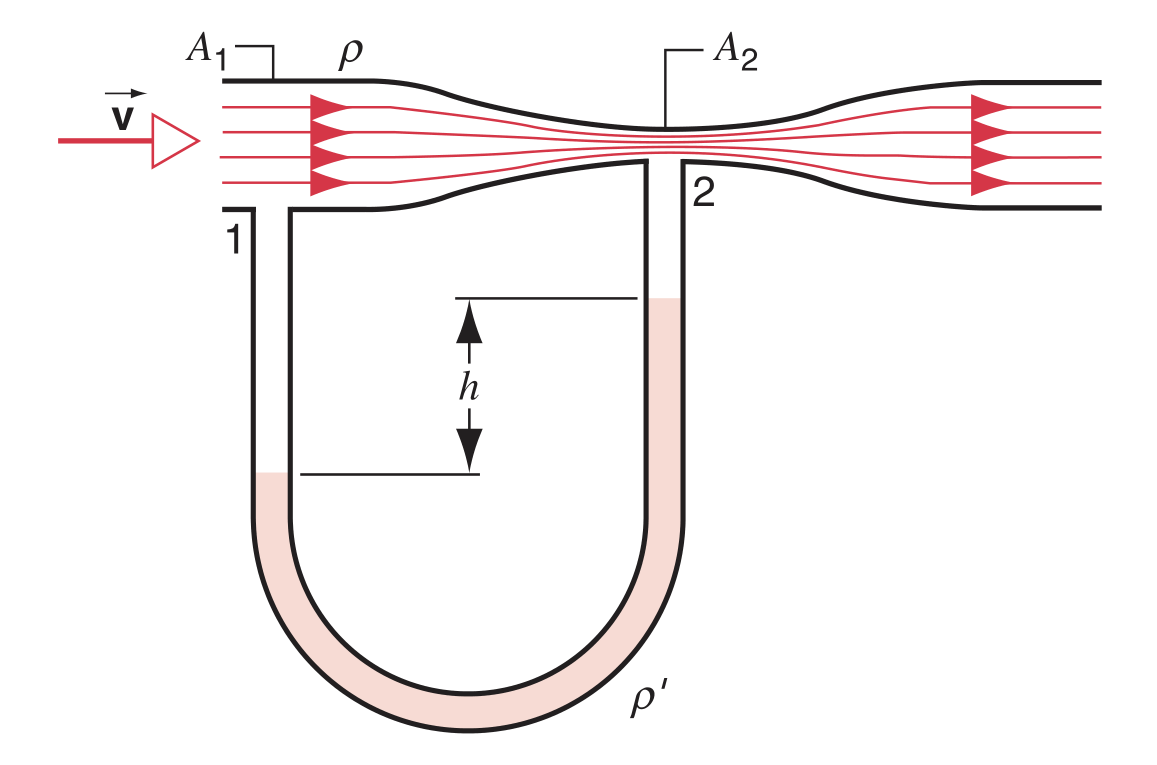
\includegraphics[width=0.7\linewidth]{images/12.venturi_meter.png}
  \caption{Venturi Meter}
  \label{fig:venturi_meter}
\end{minipage}%
\begin{minipage}{.5\textwidth}
  \centering
  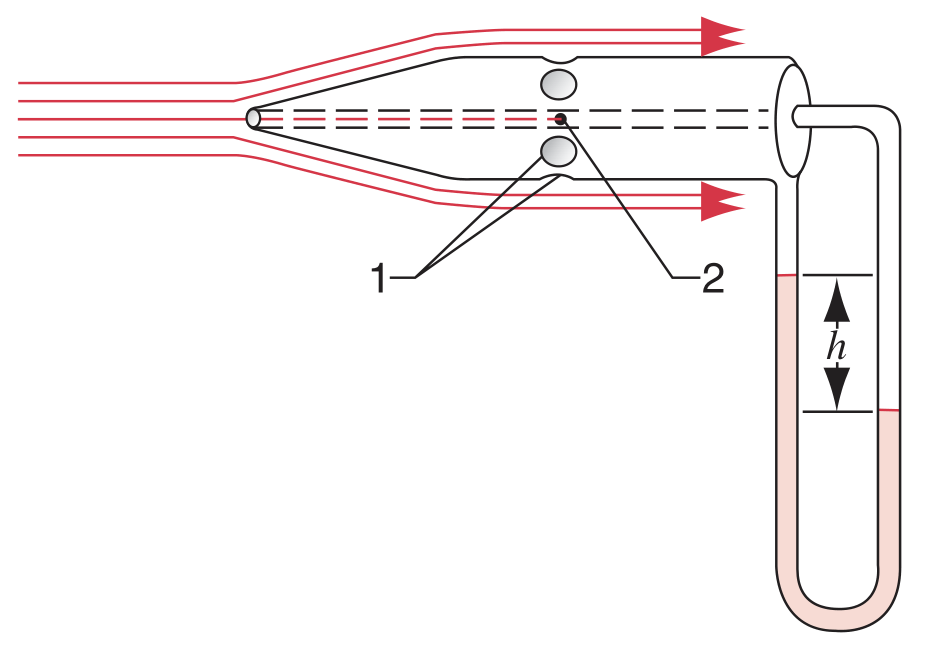
\includegraphics[width=0.7\linewidth]{images/12.pitot_tube.png}
  \caption{Pitot Tube}
  \label{fig:pitot_tube}
\end{minipage}
\end{figure}

\subsubsection{Toricelli's Law}
Toricelli's law tells us how fast a fluid will pour out of a small opening in a container at depth $h$ below the surface. 
\[ v = \sqrt{2gh} \]
To find how long it takes for a container to empty, equating volume flux (where $A_0$ is area at the surface and $A$ is area of the opening) gives us 
\[ \frac{dh}{dt} = v_0 = \frac{A}{A_0}v \]
and we need some other information to solve for $A/A_0$ before being able to solve for t. 

\subsection{Viscosity}
The viscous force is given by
\[ F = \eta A \frac{dv}{dy} \]
and the units for viscosity $\eta$ are Pascal-seconds. In liquids, viscosity results from intermolecular forces that are weakened with temperature (so, hotter means less viscous!). In gases, increased temperature means molecules migrate between layers of flow; however, there are more slow molecules than fast ones due to geometry, so this impedes faster molecules near the center (so, hotter means more viscous!).  

\subsection{Laminar Flow}
At radial distance $r$ from the center of a pipe with radius $R$, the speed is
\[ v = \frac{r \Delta p}{4 \eta L}(R^2 - r^2) \]
where $L$ is the length of the pipe and $\Delta p$ goes from its start to end. \\
The mass flux is given by
\[ Q = \frac{dm}{dt} = \frac{\pi R^4 \rho \Delta p}{8\eta L} \]
the latter of which is known as Poiseuille's Law. 

\subsection{Turbulent Flow}
Flow becomes turbulent above a critical speed, given by
\[ v_c = R\frac{\eta}{\rho D} \]
where D is the diameter of flow. For cylinders, the Reynolds number $R$ is 2300. 

\end{document}